% Appendix B
 
\chapter{Designing Figures}

This section contains recommendations on designing effective figures. We will cover graphs as well as diagrams.

\section{Fundamental Concepts}

\subsection{Layout}

% Gestalt

% alignment
% proximity
% connectedness
% 

\subsection{Color}

\section{Diagrams}

You can use diagrams to describe concepts and their relationship, the structure of systems, interactions, and (experimental) procedures.

\subsection{Common Problems}

% infohq

% examples

\subsection{Before You Start}

Questions to ask when designing a diagram:\sidenote{Taken from the book ``Designing Science Presentations: A Visual Guide to Figures, Papers, Slides, Posters, and More'' \cite{Carter12}.}
\begin{itemize}
\item What is absolutely necessary to show?
\item What is not necessary to show?
\item What is most important and should be emphasized?
\item What is not important and should be secondary to the main message?
\item What are the relationships between individual elements?
\item Does the diagram require a precise depiction of time?
\item Does the diagram require a precise depiction of distance?
\item What symbols should be consistent throughout the diagram?
\end{itemize}

\subsection{Emphasizing Elements}

Good diagrams are self-explanatory and guide the reader's attention. Humans constantly search for patterns and deviations. Consistent use of shapes and colors indicates that the presented elements are similar (cf. Fig.~\ref{fig:emphasis}). Deviation from the norm indicate differences that need attention. Be aware of that and do not create emphasis unintentionally.

\begin{figure}[t]
\centering
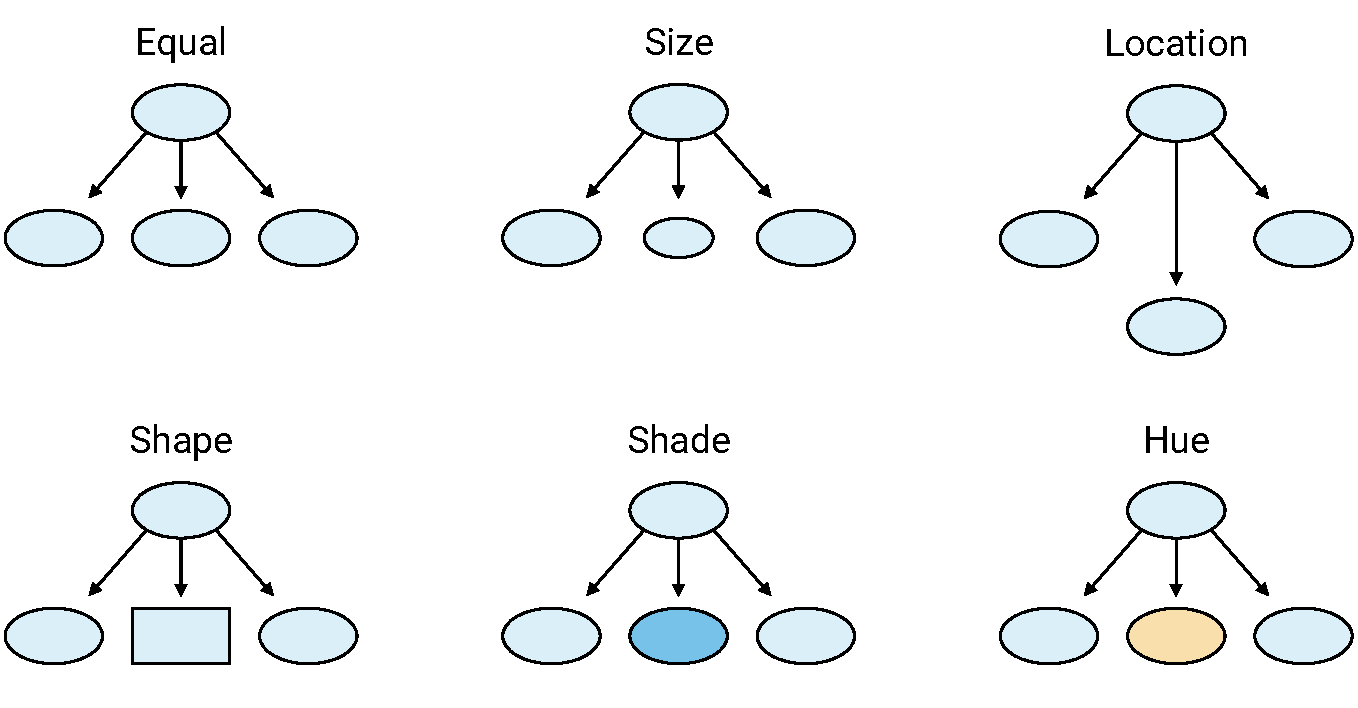
\includegraphics[width=1\textwidth]{diagram-emphasis}
\sidecaption{\label{fig:emphasis} Deviations from the norm create emphasis \cite{Carter12}.}[-4\baselineskip]
\end{figure}

Do not choose the size of elements arbitrarily. Differences translate into dominance relationships. Larger elements usually appear to control the smaller ones (cf. Fig.~\ref{fig:dominance})

\begin{figure}[t]
\centering
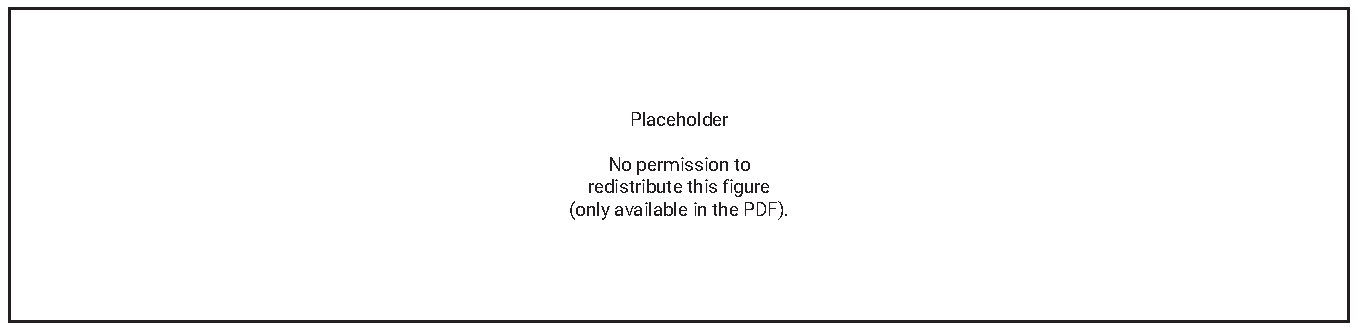
\includegraphics[width=1\textwidth]{diagram-dominance}
\sidecaption{\label{fig:dominance} Relative differences in size indicate dominance relationships \cite{Carter12}.}[-4\baselineskip]
\end{figure}

In the absence of strong emphasis, readers process diagrams similar to text (cf. Fig.~\ref{fig:direction}). In western cultures, readers will start in the top left corner and proceed horizontally in a zig-zag pattern. The general flow of information should be consistent with this expectation.

\begin{marginfigure}
\centering
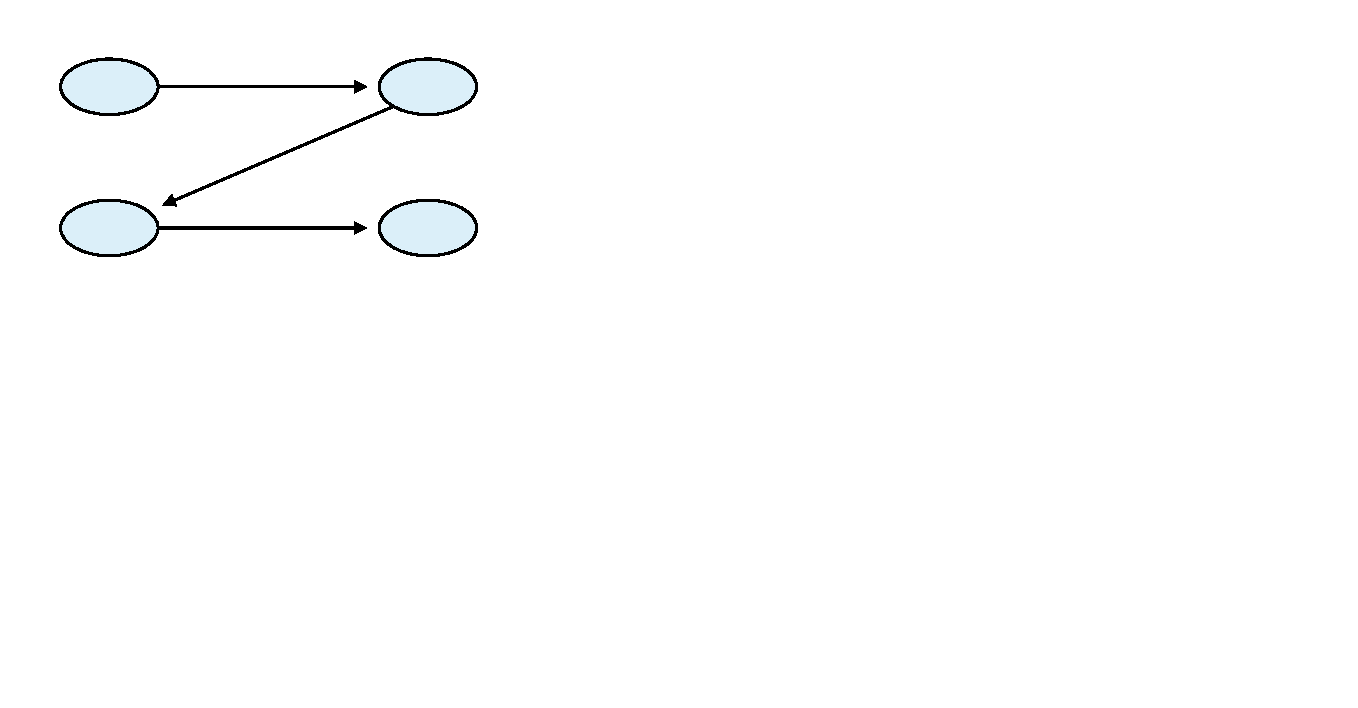
\includegraphics[width=1\textwidth]{diagram-direction}
\sidecaption{\label{fig:direction} Expected flow of information in western cultures \cite{Carter12}.}[-1\baselineskip]
\end{marginfigure}

\section{Figures}

















